\subsection{Regelkreis}

Ein Regelkreis besteht haupts\"achlich aus einem \textit{Regler} (C) und einer
Regelstreck      (engl.      \textit{Plant})     (P)     (siehe      Abbildung
\ref{fig:control-loop}).

\begin{figure}
    \centering
    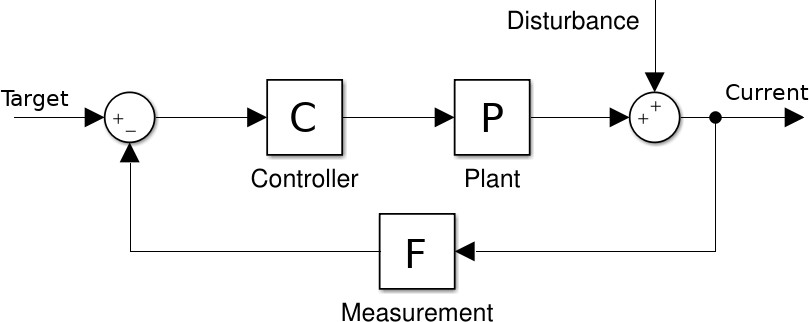
\includegraphics[width=\imagewidth]{images/control_loop}
    \caption{Aufbau eines geschlossenen Regelkreises}
    \label{fig:control-loop}
\end{figure}

Eine  unbekannte St\"orgr\"osse (engl.  \textit{Disturbance})  wirkt  auf  die
Regelstrecke, welches durch die Steuerung kompensiert werden muss.  In unserem
Fall ist die St\"orgr\"osse das  unbekannte  Lastmoment,  das  auf  den  Rotor
wirkt.

In der R\"uckkopplung befindet sich weiter die Messung des \textit{Ist}-Werts,
in  unserem Fall ist das die  Umwandlung  einer  Drehzahl  in  eine  Spannung.

Der  \textit{Ist}-Wert  wird  mit   dem   \textit{Soll}-Wert  am  Eingang  des
Regelkreises verglichen und der Regler reagiert entsprechend.

